\documentclass{article}[a4paper]
\usepackage[utf8]{inputenc}
\usepackage[spanish]{babel}
\usepackage[a4paper, 11pt]{geometry}
\usepackage{graphicx}
\newcommand{\xor}{\oplus}
%\usepackage{xcolor}
\usepackage{listings} %code highlighter
\usepackage{blindtext}
\usepackage{titlesec}
\usepackage{appendix}
\usepackage[T1]{fontenc}
\usepackage{textcomp}
\usepackage{amssymb,amsmath}
\usepackage{hyperref}
\usepackage[dvipsnames]{xcolor}
\newcommand{\dollar}{\mbox{\textdollar}}

\usepackage{listings}% http://ctan.org/pkg/listings
\lstset{
  basicstyle=\ttfamily,
  mathescape = true
}

\newcommand\tab[1][1cm]{\hspace*{#1}}

\definecolor{codegreen}{rgb}{0,0.6,0}
\definecolor{codegray}{rgb}{0.5,0.5,0.5}
\definecolor{codepurple}{rgb}{0.58,0,0.82}
\definecolor{backcolour}{rgb}{0.95,0.95,0.92}

\lstdefinestyle{mystyle}{
    backgroundcolor=\color{backcolour},   
    commentstyle=\color{codegreen},
    keywordstyle=\color{magenta},
    numberstyle=\tiny\color{codegray},
    stringstyle=\color{codepurple},
    basicstyle=\ttfamily\footnotesize,
    breakatwhitespace=false,         
    breaklines=true,                 
    captionpos=b,                    
    keepspaces=true,                 
    numbers=left,                    
    numbersep=5pt,                  
    showspaces=false,                
    showstringspaces=false,
    showtabs=false,                  
    tabsize=2
}

\lstset{style=mystyle}

\title{Memoria Práctica TDL: CompiladorG}
\author{Andrés Ollero Morales, Gabriel de Oliveira Trindade, Víctor Alejandro Sanz Ararat}
\date{Grupo 17}

\begin{document}

% \maketitle
\begin{titlepage}
   \begin{center}
       \vspace*{1cm}

       \textbf{Práctica Procesadores de Lenguajes}

       \vspace{0.5cm}
        Grupo 17
            
       \vspace{1.5cm}

        \textbf{Andrés Ollero Morales}\\
        \textbf{Víctor Alejandro Sanz Ararat}\\
        \textbf{Gabriel de Oliveira Trindade}\\

       \vfill
            
       \vspace{0.5cm}
     
       
\includegraphics[width=0.5\textwidth]{fiupm.png}

        \vfill
            
       \vspace{0.1cm}
       Departamento de Lenguajes y Sistemas Informáticos e Ingeniería de Software\\
       Escuela Técnica Superior De Ingenieros Informáticos\\
       Universidad Politécnica de Madrid\\
       Enero 2023
            
   \end{center}
\end{titlepage}
\thispagestyle{empty}
\newpage
\tableofcontents
\thispagestyle{empty}
\newpage

\section{Diseño final del Procesador}
A modo de introducción, hemos querido recordar lo que es capaz de procesar el compilador. La implementación fue realizada en el lenguaje de programación Java. Nuestro grupo contaba con las siguientes opciones de práctica:
\begin{itemize}
    \item Técnicas de Análisis Sintáctico: Descendente con tabla
    \item Sentencias: Sentencia de selección múltiple (switch-case)
    \item Operadores especiales: Asignación con resto (\%=)
    \item Comentarios: Comentario de bloque (/* */)
    \item Cadenas: Con comillas dobles (\" \")
\end{itemize}

\subsection{Diseño de Tokens}
\begin{verbatim}
        <palabraReservada, boolean>         <palabraReservada, input>
        <palabraReservada, break>           <palabraReservada, int>
        <palabraReservada, case>            <palabraReservada, let>
        <palabraReservada, function>        <palabraReservada, switch>
        <palabraReservada, print>           <palabraReservada, return>
        <palabraReservada, string>          <palabraReservada, if>
        <palabraReservada, default>
        
        <suma, >            <puntoComa, >       <asignacion, >
        <negacion, >        <coma, >            <dosPuntos, >
        <abrePar, >         <cierraPar, >       <comparacion, >
        <abreLlave, >       <cierraLlave, >     <asignacionResto, >
        <id, nºTS>          <constEnt, nº>      <cadena, "lexema">
\end{verbatim}

%\begin{figure}[h!]
%\centering
%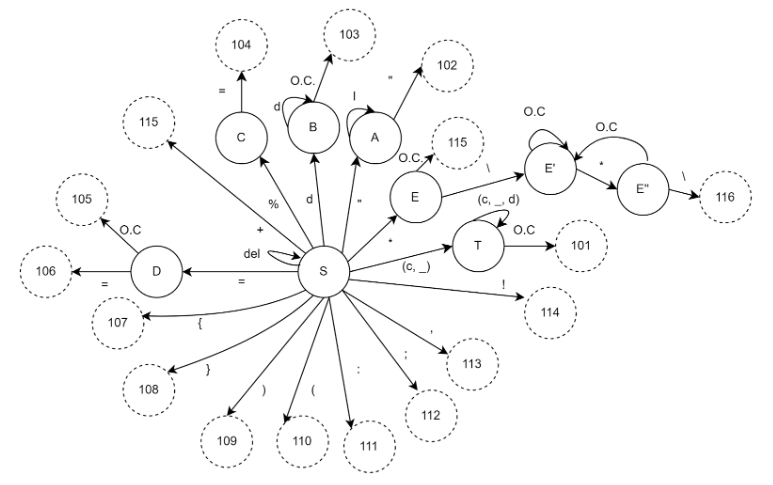
\includegraphics[width=0.9\textwidth]{automataAnLex.png}
%\caption{\label{figura:automata}Implementación de la gramática con el autómata.}
%\end{figure}

\subsection{Gramática de Contexto Libre (Tipo II)}
Esta gramática es sobre la que hacemos las acciones semánticas mediante Traducción Dirigida por la Sintáxis.

\begin{verbatim}
Axioma = PP

NoTerminales = { PP P S SS E R RR U UU V VV L Q X B T A K C F H O D }

Terminales = { ! == + id ( ) constEnt cadena %= print input return , if break 
                switch case int boolean string let function ; : = { } default }

Producciones = {
    E -> R RR
    RR -> == R RR
    RR -> lambda
    R -> U UU
    UU -> + U UU
    UU -> lambda
    U -> ! V
    U -> V
    V -> id VV
    V -> ( E )
    V -> constEnt
    V -> cadena
    VV -> ( L )
    VV -> lambda
    S -> id SS
    SS -> %= E ;
    SS -> = E ;
    SS -> ( L ) ;
    S -> print R ;
    S -> input id ;
    S -> return X ;
    L -> E Q
    L -> lambda
    Q -> , E Q
    Q -> lambda
    X -> E
    X -> lambda
    B -> switch ( E ) { O }
    B -> if ( E ) S
    O -> case constEnt : C D O
    O -> default : C D O
    O -> lambda
    D -> break ;
    D -> lambda
    B -> let id T ;
    T -> int
    T -> boolean
    T -> string
    B -> S
    F -> function id H ( A ) { C }
    H -> T
    H -> lambda
    A -> T id K
    A -> lambda
    K -> , T id K
    K -> lambda
    C -> B C
    C -> lambda
    P -> B P
    P -> F P
    P -> lambda
    PP -> P
}
\end{verbatim}

\newpage

\section{Diseño del Generador de Código Intermedio}

\subsection{Traducción Dirigida Por la Sintáxis con Acciones Semánticas}

Aprovechamos el diseño del Esquema de Traducción del procesador para añadir las nuevas acciones semánticas del Generador de Código Intermedio. A continuación se muestra una breve descripción de todas los métodos y funciones que aparecen en las acciones.\\

\noindent\textbf{Métodos:}\\
\tab emite(operador, op1, op2, res): Escribe en el fichero de código intermedio la operación descrita por el cuarteto (algunos operandos pueden valer nulo).\\
\tab buscaEtTS(idPos): Busca la etiqueta por la posición de la Tabla de Símbolos correspondiente del id que la representa.\\
\tab nuevaEt(): Crea una nueva etiqueta en la Tabla de Símbolos.\\
\tab tamRAcalculator(): Calcula cuánto ocupa el tamaño del Registro de Activación de una función en pila.\\
\tab buscaTipoTS(idPos): Busca el tipo de un id según su posición en la Tabla de Símbolos correspondiente.\\
\tab buscaLugarTS(idPos): Busca la posición en la Tabla de Símbolos correspondiente el id determinado.\\

\noindent\textbf{Atributos de los No Terminales:}\\
\tab .evaluado: Determina si el case de un switch ya ha sido evaluado, para así no hacer las comprobaciones de los siguientes cases y los ejecute directamente si no hay break en dicho case.\\
\tab .siguiente: \\
\tab .pos: Determina cuál es la posicion dentro de una tabla de símbolos\\
\tab .lugar: Determina cuál es el lugar de la variable dentro de una tabla de símbolos\\
\tab .break: Determina la etiqueta a la que se debe saltar dentro de un switch para saltar fuera del switch cuando se encuentra un break\\
\tab .tipo: Determina el tipo del no terminal correspondiente\\
\tab .etiq: Determina cual es la etiqueta que tiene una función o una string\\
\tab .params: Es un Array que contiene el lugar de los parámetros que se van a pasar a la llamada a función siguiente\\

\noindent\underline{Bloque Axioma:}\\

\tab PP $\rightarrow$ P \textcolor{OliveGreen}{$ $\lbrace$Ø$\rbrace$_{1}$}\\

\tab P $\rightarrow$ B P \textcolor{OliveGreen}{$ $\lbrace$Ø$\rbrace$_{2}$}\\

\tab P $\rightarrow$ F P \textcolor{OliveGreen}{$ $\lbrace$Ø$\rbrace$_{3}$}\\

\tab P $\rightarrow$ $\lambda$ \textcolor{OliveGreen}{$ $\lbrace$Ø$\rbrace$_{4}$}\\ 

\noindent\underline{Bloque declaración de funciones:}\\

\tab F $\rightarrow$ function id 
H ( A ) \textcolor{OliveGreen}{$ $\lbrace$emite(‘:’, buscaEtTS(id.pos), NULL, NULL)$\rbrace$_{5.2}$} \\ \tab \tab
$\lbrace$ C  \textcolor{OliveGreen}{$ $\lbrace$tamRAcalculator()$\rbrace$_{5.3}$} $\rbrace$ \textcolor{OliveGreen}{$ $\lbrace$emite(‘return’, NULL, NULL, NULL)$\rbrace$_{5.4}$}\\

\tab H $\rightarrow$ T \textcolor{OliveGreen}{$ $\lbrace$Ø$\rbrace$_{6}$}\\

\tab H $\rightarrow$ $\lambda$ \textcolor{OliveGreen}{$ $\lbrace$Ø$\rbrace$_{7}$}\\

\tab A $\rightarrow$ T id K \textcolor{OliveGreen}{$ $\lbrace$Ø$\rbrace$_{8}$}\\

\tab A $\rightarrow$ $\lambda$ \textcolor{OliveGreen}{$ $\lbrace$Ø$\rbrace$_{9}$}\\

\tab K $\rightarrow$ , T id K \textcolor{OliveGreen}{$ $\lbrace$Ø$\rbrace$_{10}$}\\

\tab K $\rightarrow$ $\lambda$ \textcolor{OliveGreen}{$ $\lbrace$Ø$\rbrace$_{11}$}\\

\tab C $\rightarrow$ B C \textcolor{OliveGreen}{$ $\lbrace$Ø$\rbrace$_{12}$}\\

\tab C $\rightarrow$ $\lambda$ \textcolor{OliveGreen}{$ $\lbrace$Ø$\rbrace$_{13}$}\\

\noindent\underline{Bloque sentencias compuestas y declaración de variables:}\\

\tab B $\rightarrow$ if ( E ) \textcolor{OliveGreen}{$ $\lbrace$B.siguiente := nuevaEt(), emite(‘if’, E.lugar, NULL, B.siguiente)$\rbrace$_{14.1}$}\\
\tab \tab \tab S \textcolor{OliveGreen}{$ $\lbrace$emite(‘:’, B.siguiente, NULL, NULL)$\rbrace$_{14}$}\\

%-----------------------SWITCH XD-----------------------------------------

\tab B $\rightarrow$ switch ( E ) 
$\lbrace$ O $\rbrace$ \textcolor{OliveGreen}{$ $\lbrace$emite(‘:’, B.break, NULL, NULL)$\rbrace$_{15.3}$}\\

\tab O $\rightarrow$ case constEnt \textcolor{OliveGreen}{$ $\lbrace$
O.break := B.break, O.evaluado := B.evaluado \\
\tab \tab \tab \tab O.siguiente := nuevaEtiq(), O.lugar := E.lugar \\
\tab \tab \tab \tab emite(‘if==’, B.evaluado, 1, sig\_inst + 1) \\
\tab \tab \tab \tab emite(‘if!=’, O.lugar, constEnt, O.siguiente)
$\rbrace$_{16.1}$} \\ \tab \tab
 : C D \textcolor{OliveGreen}{$ $\lbrace$emite(‘:’, 1, NULL, O.evaluado)
emite(‘:’, O.siguiente, NULL, NULL)$\rbrace$_{16.3}$}\\
\tab \tab O \textcolor{OliveGreen}{$ $\lbrace$Ø$\rbrace$_{16.2}$}\\

%-----------------------SWITCH XD-----------------------------------------
   
\tab O $\rightarrow$ $\lambda$ \textcolor{OliveGreen}{$ $\lbrace$Ø$\rbrace$_{18}$}\\

\tab D $\rightarrow$ break ; \textcolor{OliveGreen}{$ $\lbrace$emite(‘goto’, D.break, NULL, NULL)$\rbrace$_{19}$}\\

\tab D $\rightarrow$ $\lambda$ \textcolor{OliveGreen}{$ $\lbrace$Ø$\rbrace$_{20}$}\\

\tab B $\rightarrow$ let id T ; \textcolor{OliveGreen}{$ $\lbrace$Ø$\rbrace$_{21}$}\\

\tab T $\rightarrow$ int \textcolor{OliveGreen}{$ $\lbrace$Ø$\rbrace$_{22}$}\\

\tab T $\rightarrow$ boolean \textcolor{OliveGreen}{$ $\lbrace$Ø$\rbrace$_{23}$}\\

\tab T $\rightarrow$ string \textcolor{OliveGreen}{$ $\lbrace$Ø$\rbrace$_{24}$}\\

\tab B $\rightarrow$ S \textcolor{OliveGreen}{$ $\lbrace$Ø$\rbrace$_{25}$}\\ \\ \\

\noindent\underline{Sentencias simples:}\\

\tab S $\rightarrow$ id SS \textcolor{OliveGreen}{$ $\lbrace$SS.tipo := BuscaTipoTS(id.pos)\\ \tab \tab \tab \tab
SS.lugar := BuscaLugarTS(id.pos) \\ \tab \tab \tab \tab 
if SS.tipo == funcion then SS.etiq := BuscaEtiqTS(id.pos)$\rbrace$_{26}$}\\

 \tab SS $\rightarrow$ \%= E ; \textcolor{OliveGreen}{$ $\lbrace$emite(‘\%’, E.lugar, SS.lugar, SS.lugar)$\rbrace$_{27}$}\\

\tab SS $\rightarrow$ = E ; \textcolor{OliveGreen}{$ $\lbrace$emite(‘:=’, E.lugar, NULL, SS.lugar)$\rbrace$_{28}$}\\

\tab SS $\rightarrow$ ( L ) ;  \textcolor{OliveGreen}{$ $\lbrace$for (param in L.params) \\ \tab \tab \tab \tab \tab
emite(‘param’, param, NULL, NULL) \\ \tab \tab \tab \tab
emite(‘call’,SS.etiq, NULL, NULL)$\rbrace$_{29}$}\\

\tab S $\rightarrow$ print R ;  \textcolor{OliveGreen}{$ $\lbrace$emite(“print”, R.lugar, NULL, NULL)$\rbrace$_{30}$}\\

\tab S $\rightarrow$ input id ; \textcolor{OliveGreen}{$ $\lbrace$emite(“input”, BuscaLugarTS(id), NULL, NULL)$\rbrace$_{31}$}\\

\tab S $\rightarrow$ return X ; \textcolor{OliveGreen}{$ $\lbrace$emite(‘return’, X.lugar, NULL, NULL)$\rbrace$_{32}$}\\

\tab L $\rightarrow$ E Q \textcolor{OliveGreen}{$ $\lbrace$L.param := E.lugar \bigoplus Q.param$\rbrace$_{33}$}\\
	
 \tab L $\rightarrow$ $\lambda$ \textcolor{OliveGreen}{$ $\lbrace$Ø$\rbrace$_{34}$}\\ 

\tab Q $\rightarrow$ , E Q1 \textcolor{OliveGreen}{$ $\lbrace $Q.param := E.lugar \bigoplus Q1.param$\rbrace$_{35}$}\\

\tab Q $\rightarrow$ $\lambda$ \textcolor{OliveGreen}{$ $\lbrace$Ø$\rbrace$_{36}$}\\

\tab X $\rightarrow$ E \textcolor{OliveGreen}{$ $\lbrace$X.lugar := E.lugar$\rbrace$_{37}$}\\

\tab X $\rightarrow$ $\lambda$ \textcolor{OliveGreen}{$ $\lbrace$Ø$\rbrace$_{38}$}\\


\noindent\underline{Expresiones:}\\

\tab E $\rightarrow$ R RR \textcolor{OliveGreen}{$ $\lbrace$
if RR.tipo != vacio\\ \tab \tab \tab \tab
then E.lugar := nuevaTemp(logico)\\ \tab \tab \tab 
emite(‘if==’, R.lugar, RR.lugar, goto 2)\\  \tab \tab \tab 
emite(‘:=’, 0, null, E.lugar)\\ \tab \tab \tab 
emite(‘goto’, sigInst + 1)\\ \tab \tab \tab 
emite(‘:=’, 1, null, E.lugar))\\ \tab \tab \tab 
else then \\ \tab \tab \tab \tab
E.lugar := R.lugar\\ \tab \tab \tab 
emite(‘:=’, R.lugar, null, E.lugar)$\rbrace$_{39}$}\\

\tab RR $\rightarrow$ == R RR \textcolor{OliveGreen}{$ $\lbrace$RR.lugar := R.lugar$\rbrace$_{40}$}\\

\tab RR $\rightarrow$ $\lambda$ \textcolor{OliveGreen}{$ $\lbrace$Ø$\rbrace$_{41}$}\\

 \tab R $\rightarrow$ U UU \textcolor{OliveGreen}{$ $\lbrace$UU.lugar := nuevaTemp(constEnt) \\ \tab \tab \tab \tab
if UU1.tipo == vacio \\ \tab \tab \tab \tab \tab
then emite(‘:=’, U.lugar, null, UU.lugar) \\ \tab \tab \tab \tab
else \\ \tab \tab \tab \tab \tab
then emite(‘+’, U.lugar, UU1.lugar, UU.lugar)$\rbrace$_{43}$}\\

 \tab UU $\rightarrow$ + U UU \textcolor{OliveGreen}{$ $\lbrace$if (U.tipo = constEnt \&\& UU2.tipo != tipo.error)\\ \tab \tab \tab \tab \tab
then UU.tipo := tipo.ok\\ \tab \tab \tab \tab
else then UU.tipo := tipo.error\\ \tab \tab \tab \tab \tab
error(“error semantico: operando solo admite valores enteros”);\\ \tab \tab \tab \tab
POP(3)$\rbrace$_{44}$}\\

\tab UU $\rightarrow$ $\lambda$ \textcolor{OliveGreen}{$ $\lbrace$Ø$\rbrace$_{45}$}\\

 \tab U $\rightarrow$ ! V \textcolor{OliveGreen}{$ $\lbrace$U.lugar := nuevaTemp(boolean)\\ \tab \tab \tab \tab
 emite(‘not’, V.lugar, NULL, U.lugar$\rbrace$_{46}$}\\

 \tab U $\rightarrow$ V \textcolor{OliveGreen}{$ $\lbrace$U.lugar := V.lugar$\rbrace$_{47}$}\\

 \tab V $\rightarrow$ id VV \textcolor{OliveGreen}{$ $\lbrace$if buscaTipoTS(id.pos) != function\\  \tab \tab \tab \tab
then V.lugar := buscaLugarTS(id.pos)\\ \tab \tab \tab 
else then \\ \tab \tab \tab \tab 
VV.etiq := BuscaEtiqTS(id.pos)\\ \tab \tab \tab \tab
V.lugar = VV.lugar$\rbrace$_{48}$}\\

\tab V $\rightarrow$ ( E ) \textcolor{OliveGreen}{$ $\lbrace$V.lugar := E.lugar$\rbrace$_{49}$}\\

 \tab V $\rightarrow$ constEnt \textcolor{OliveGreen}{$ $\lbrace$V.lugar := nuevaTemp(tipo.constEnt);\\ \tab \tab \tab \tab
 emite(‘:=’, constEnt.valor, NULL, V.lugar)$\rbrace$_{50}$}\\

 \tab V $\rightarrow$ cadena \textcolor{OliveGreen}{$ $\lbrace$V.lugar := nuevaTemp(tipo.cadena);\\ \tab \tab \tab \tab
 emite(‘:=’, cadena.etiqueta, NULL, V.lugar)$\rbrace$_{51}$}\\

 \tab VV $\rightarrow$ ( L )  \textcolor{OliveGreen}{$ $\lbrace$VV = nuevaTemp() \\ \tab \tab \tab \tab
for (param in L.params) \\ \tab \tab \tab \tab \tab
emite(‘param’, param, NULL, NULL) \\ \tab \tab \tab \tab
emite(‘call’, VV.etiq, NULL, VV.lugar)$\rbrace$_{52}$}\\

 \tab VV $\rightarrow$ $\lambda$ \textcolor{OliveGreen}{$ $\lbrace$Ø$\rbrace$_{53}$}\\

\newpage

\section{Diseño del Generador de Código Final}

\subsection{Plantilla de Traducción de Cuartetos}

A continuación se muestran todos los posibles cuartetos generados por el Generador de Código Intermedio, y su correspondiente traducción a Código Objeto. Nótese que para cada operando que aparece en el cuarteto, se recogerá la dirección del mismo de una forma u otra (puede ser una constante, o estar en alguan tabla de símbolos...). También algunas traducciones pueden variar dependiendo del caso en el que estemos ejecutando (dentro de una función o desde main).\\

Emitiremos la traducción a ensamblador en el momento en el que se haga un emite del código intermedio.

\begin{itemize}

\item (+, op1, op2, res)
\begin{verbatim}
    ADD op1, op2
    MOVE .A, res
\end{verbatim}\\

\item (:=, op1, NULL, res)
\begin{verbatim}
    MOVE op1, res
\end{verbatim}\\

\item (:, et01, null, null)
\begin{verbatim}
    et01: NOP
\end{verbatim}\\

\item (\%, op1, op2, res)
\begin{verbatim}
    MOD op1, op2
    MOVE .A, res
\end{verbatim}\\

\item (print, op1, null, null)\\
En el caso de que sea una string:
\begin{verbatim}
    ADD #0, op1
    WRSTR [.A]
\end{verbatim}
Accedemos accedemos a lo que apunta el acumulador, ya que es una etiqueta a una string.

En el caso de que sea un entero:
\begin{verbatim}
    WRINT op1
\end{verbatim}

\item (input, op1, null, null)\\
En el caso de que sea una string:
\begin{verbatim}
    INSTR op1
\end{verbatim}
En el caso de que sea un entero:
\begin{verbatim}
    ININT op1
\end{verbatim}

\item (return, op1, null, null)
\begin{verbatim}
    SUB #Tam_RA_X, #1
    ADD .A, .IX
    MOVE op1, [.A]
    BR [.IX]
\end{verbatim}

\item (return, op1, null, null)
\begin{verbatim}
    BR [.IX]
\end{verbatim}

\item (not, op1, null, res)
\begin{verbatim}
    XOR op1, #1
    MOVE .A, res
\end{verbatim}

\item (goto, null, null, sig\_int + 1)
\begin{verbatim}
    BR $3
\end{verbatim}

\item (goto, et1, null, null)
\begin{verbatim}
    BR /et1
\end{verbatim}

\item (if, op1, null, et01)
\begin{verbatim}
    CMP op1, #1
    BNZ /et01
\end{verbatim}

\item (if==, op1, op2, 2)
\begin{verbatim}
    CMP op1, op2
    BZ $5
\end{verbatim}

\item (if!=, op1, constEnt, et01)
\begin{verbatim}
    CMP op1, constEnt
    BNZ /et01
\end{verbatim}

\item (call, et1, null, res)
\begin{verbatim}
    ADD #Tam_RA_X, .IX
    MOVE #dir_ret_X, [.A] 
    MOVE .A, .IX
    BR /etX
    dir_ret_X: NOP
    SUB #Tam_RA_X, #1
    ADD .A, .IX
    MOVE [.A], .R9
    SUB .IX, #Tam_RA_X
    MOVE .A, .IX
    MOVE .R9, res
\end{verbatim}

\item (call, et1, null, null)
\begin{verbatim}
    ADD #Tam_RA_X, .IX
    MOVE #dir_ret_X, [.A] 
    MOVE .A, .IX
    BR /etX
    dir_ret_X: NOP
    SUB .IX, #Tam_RA_X
    MOVE .A, .IX
\end{verbatim}

\item (param, op1, null, null)
\begin{verbatim}
    ADD #0, .IX
    ADD #desp, .A
    MOVE op1, [.A]
\end{verbatim}

\end{itemize}




\subsection{Tratamiento de las Strings}
Las strings se tratan de manera que cada cadena de texto se almacena en el ensamblador con una etiqueta generada, esto es posible gracias a la instrucción DATA, en el caso de que la cadena este implícita en el código. \\ \\
En el caso en el que la cadena es recibida por medio de input, se reservan 64 espacios de memoria con la instrucción RES 64 y una etiqueta para que se almacenene la string. \\ \\
Todas las cadenas se inicializan a la string vacia, \"\".

\section{Diseño del Entorno de Ejecución}

\subsection{Esquema de la memoria en ejecución}
La asignación de la memoria se realiza como describe la siguiente figura:\\

\begin{figure}[h!]
\centering
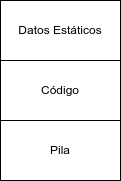
\includegraphics[width=0.2\textwidth]{EE.png}
\caption{\label{figura:EE}Estructuración de las zonas de memoria.}
\end{figure}

La primera parte de la memoria será la zona de Datos Estáticos, en donde se cargarán variables globales y datos temporales de la ejecución de main. La segunda zona son las instrucciones en ensamblador. E inmediatamente debajo de ellas, está la zona de pila, que comienza justo después de la última instruccion emitida, y carga todos los Registros de Activación a partir de ellas. Esta última crece hacia posiciones crecientes de memoria.\\

Utilizamos los registros .IX para acceder a la zona de pila, y .IY para la zona de datos estáticos, ya que estos aceptan direccionamientos relativos.

\subsection{Diseño del Registro de Activación}

El Registro de Activación será apilado en la zona de memoria de la pila una consecutivamente de la otra. Está compuesto de los siguientes campos:

\begin{itemize}
    \item Estado de la máquina: Contiene la información necesaria para restaurar la ejecución por donde se dejó antes de la llamada a la subrutina. En nuestro caso solo contendrá la dirección de retorno.
    \item Parámetros: Contiene los valores necesarios con los que se inicializan los parámetros que utiliza la función.
    \item Variables Locales: Todas las variables que se declaren en la función, se almacenarán sus valores en este campo.
    \item Datos Temporales: Aquí se almacenarán valores como constantes enteras, operaciones aritméticas o evaluaciones de condiciones booleanas o de parámetros a llamadas de otras funciones. 
    \item Valor Devuelto: El llamado cargará en este campo el valor devuelto 
\end{itemize}

\begin{figure}[h!]
\centering
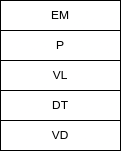
\includegraphics[width=0.2\textwidth]{RA.png}
\caption{\label{figura:RA}Campos del Registro de Activación.}
\end{figure}

Los campos EM y P los carga el llamante, el resto los usa la propia función llamada. Y el valor devuelto se encarga de ubicarlo el llamado, para que lo pueda recojer el llamante posteriormente. En la práctica, los campos de variables locales y datos temporales se entremezclan entre ellos, ya que la función los utiliza de forma indiscriminada.

\newpage
\begin{appendices}

\section{Casos de Prueba}

\subsection{Prueba Funcional 1}

Código fuente:
\lstinputlisting[language=JavaScript]{pruebas/ejemplo2/fuente.txt}\\
\hspace{\parindent} Fichero de lenguaje intermedio generado:
\lstinputlisting[language=JavaScript]{pruebas/ejemplo2/gci.txt}\\
\hspace{\parindent} Fichero de lenguaje objeto generado:
\lstinputlisting[language=JavaScript]{pruebas/ejemplo2/objeto.txt}\\
\hspace{\parindent} Fichero de Tabla de simbolos generado:
\lstinputlisting[language=JavaScript]{pruebas/ejemplo2/ts.txt}\\

En este primer ejemplo probamos la declaración de variables, la asignación, con y sin resto, 
las comparaciones y los "if" simples, asi como el print.

\subsection{Prueba Funcional 2}

Código fuente:
\lstinputlisting[language=JavaScript]{pruebas/ejemplo1/fuente.txt}\\
\hspace{\parindent} Fichero de lenguaje intermedio generado:
\lstinputlisting[language=JavaScript]{pruebas/ejemplo1/gci.txt}\\
\hspace{\parindent} Fichero de lenguaje objeto generado:
\lstinputlisting[language=JavaScript]{pruebas/ejemplo1/objeto.txt}\\
\hspace{\parindent} Fichero de Tabla de simbolos generado:
\lstinputlisting[language=JavaScript]{pruebas/ejemplo1/ts.txt}\\

En este segundo ejemplo probamos la declaración de variables, el print de cadenas, las llamadas a funciones que retornan valor, y el uso de print de un entero con llamada a una función.

\subsection{Prueba Funcional 3}

Código fuente:
\lstinputlisting[language=JavaScript]{pruebas/ejemplo3/fuente.txt}\\
\hspace{\parindent} Fichero de lenguaje intermedio generado:
\lstinputlisting[language=JavaScript]{pruebas/ejemplo3/gci.txt}\\
\hspace{\parindent} Fichero de lenguaje objeto generado:
\lstinputlisting[language=JavaScript]{pruebas/ejemplo3/objeto.txt}\\
\hspace{\parindent} Fichero de Tabla de simbolos generado:
\lstinputlisting[language=JavaScript]{pruebas/ejemplo3/ts.txt}\\

En este ejemplo realizamos varias pruebas de llamada a funciones, con input's de string y print de ellos, además de probar el funcionamiento de tanto variables locales como globales.

\subsection{Prueba Funcional 4}

Código fuente:
\lstinputlisting[language=JavaScript]{pruebas/ejemplo4/fuente.txt}\\
\hspace{\parindent} Fichero de lenguaje intermedio generado:
\lstinputlisting[language=JavaScript]{pruebas/ejemplo4/gci.txt}\\
\hspace{\parindent} Fichero de lenguaje objeto generado:
\lstinputlisting[language=JavaScript]{pruebas/ejemplo4/objeto.txt}\\
\hspace{\parindent} Fichero de Tabla de simbolos generado:
\lstinputlisting[language=JavaScript]{pruebas/ejemplo4/ts.txt}\\

En este ejemplo realizamos llamadas recursivas a una función para probar el correcto funcionamiento de la recursividad.

\subsection{Prueba Funcional 5}

Código fuente:
\lstinputlisting[language=JavaScript]{pruebas/ejemplo5/fuente.txt}\\
\hspace{\parindent} Fichero de lenguaje intermedio generado:
\lstinputlisting[language=JavaScript]{pruebas/ejemplo5/gci.txt}\\
\hspace{\parindent} Fichero de lenguaje objeto generado:
\lstinputlisting[language=JavaScript]{pruebas/ejemplo5/objeto.txt}\\
\hspace{\parindent} Fichero de Tabla de simbolos generado:
\lstinputlisting[language=JavaScript]{pruebas/ejemplo5/ts.txt}\\

En esta prueba se realiza todo tipo de operaciones, como sumas con llamadas a funciones, comparaciones con llamadas a funciones, switch sin break, anidamiento de funciones, entre otras cosas.

\end{appendices}

\end{document}